\documentclass{if-beamer}



% --------------------------------------------------- %
%                  Presentation info	              %
% --------------------------------------------------- %
\title[microAutoware: Autoware para microcontroladores]{Arquitetura HIL para teste de sistemas embarcados como \textit{vehicle interface} de veículos autônomos baseados no Autoware}
\subtitle{Projeto -- Apresentação final}

\author[Gabriel Toffanetto]{\texorpdfstring
	{Gabriel Toffanetto França da Rocha 
		\\ \vspace{1mm} 
		\small{\href{mailto:g289320@dac.unicamp.br}{g289320@dac.unicamp.br}}
	}
	{Gabriel Toffanetto França da Rocha}
}

\institute[LMA/FEM/Unicamp]{\small{Professor Dr. Rodrigo Moreira Bacurau
  \\ \vspace{2mm}
  IM420X -- Projeto de Sistemas Embarcados de Tempo Real
  \\ \vspace{4mm}
  Faculdade de Engenharia Mecânica
  \\ \vspace{1mm}
  Universidade Estadual de Campinas}
}

\date{26 de novembro de 2024}

\logo{
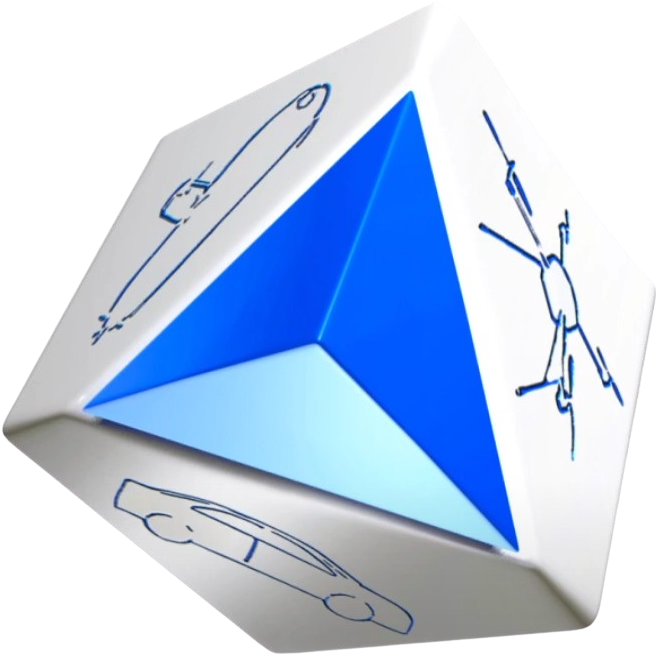
\includegraphics[width=1.2cm]{img/core/Logo_LMA_icon.png}
}


\subject{IM420X - Projeto final - microAutoware: Autoware para microcontroladores} % metadata

\graphicspath{{img/}}

\setbeamertemplate{caption}[numbered]

\newcolumntype{b}{>{\columncolor{white}}c}


\hypersetup{pdfpagemode=FullScreen}


% --------------------------------------------------- %
%                    Title + Schedule                 %
% --------------------------------------------------- %

\begin{document}

\begin{frame}
  \titlepage
\end{frame}

\begin{frame}{Agenda}
  \tableofcontents
\end{frame}

% --------------------------------------------------- %
%                      Presentation                   %
% --------------------------------------------------- %

\section{Introdução}

\begin{frame}{Contextualização}
	
	\begin{columns}
		
		\begin{column}{0.45\textwidth}
			
			
			\begin{figure}[H]
				\centering
				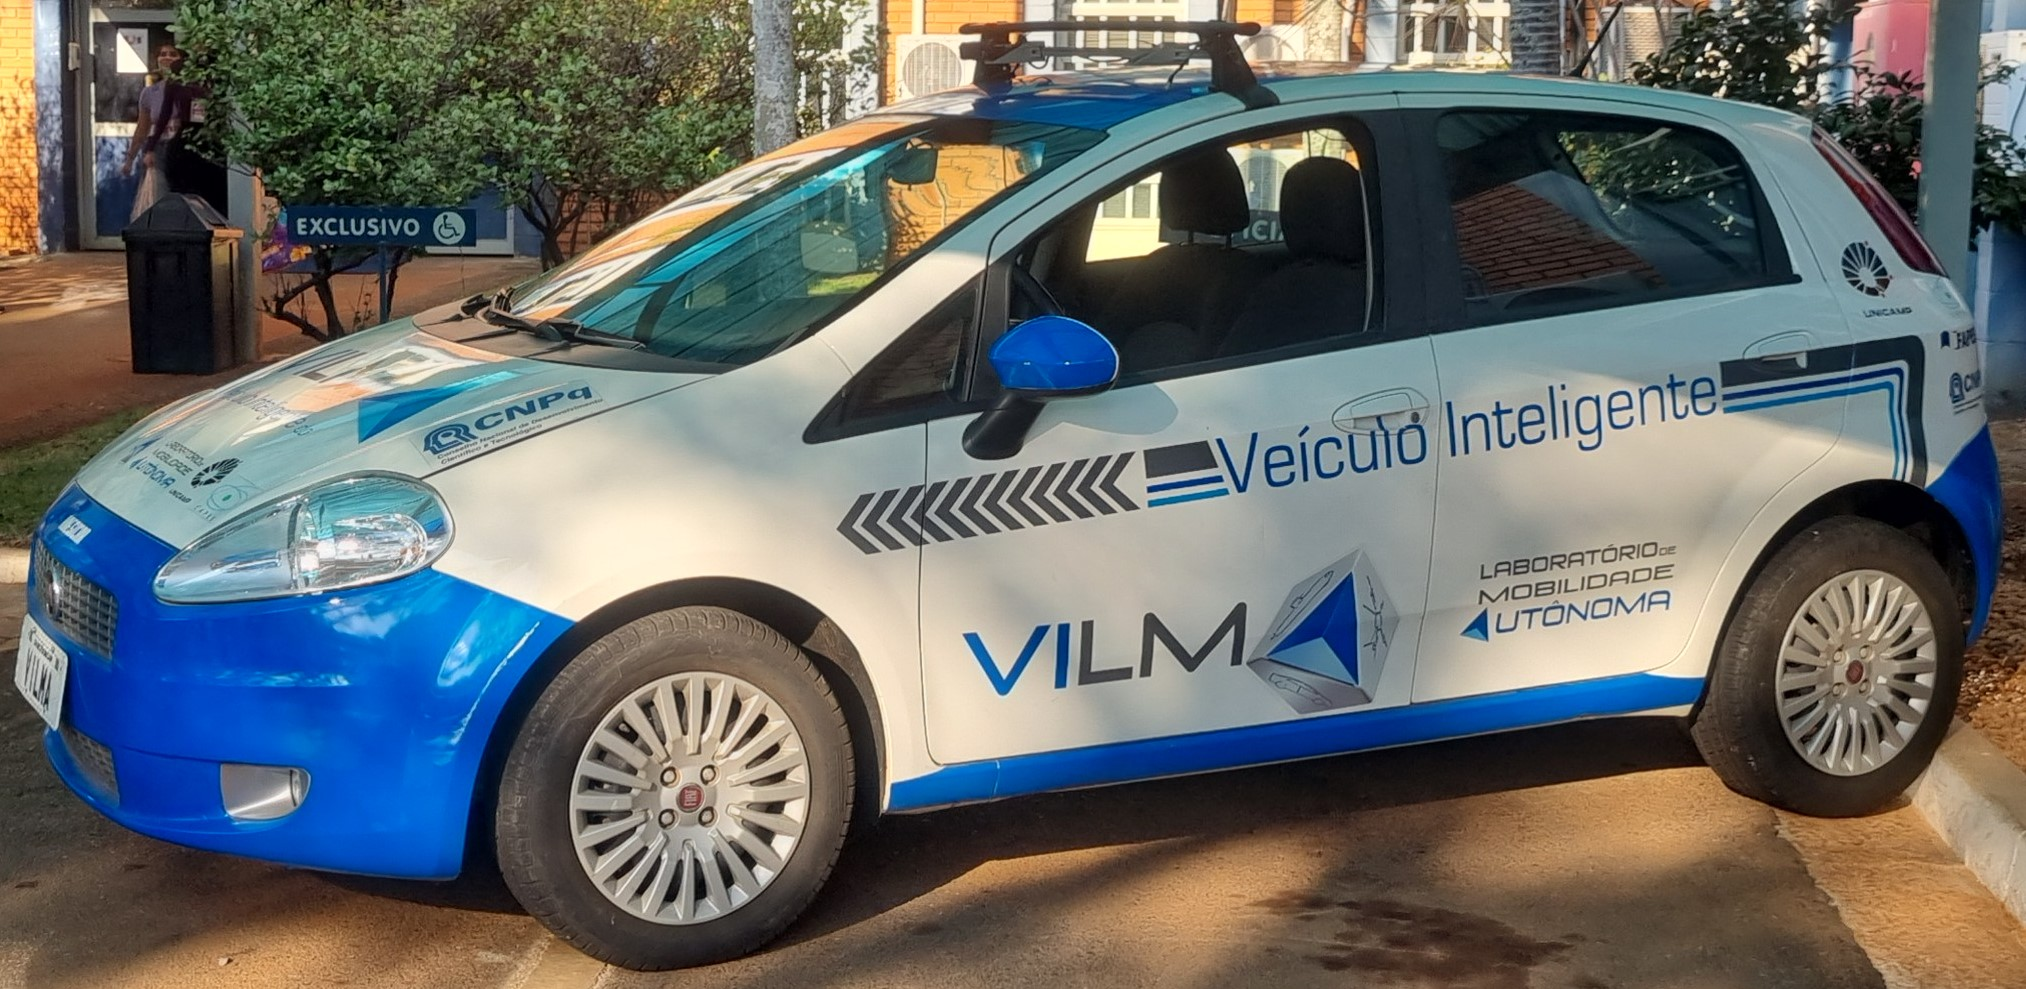
\includegraphics[width=1\linewidth]{img/vilma}
				\caption{Veículo Autônomo do LMA.}
				\label{fig:vilma}
			\end{figure}
		\end{column}
		
		\hspace{-0.5cm}
		
		\begin{column}{0.6\textwidth}
			
			\begin{figure}[H]
				\centering
				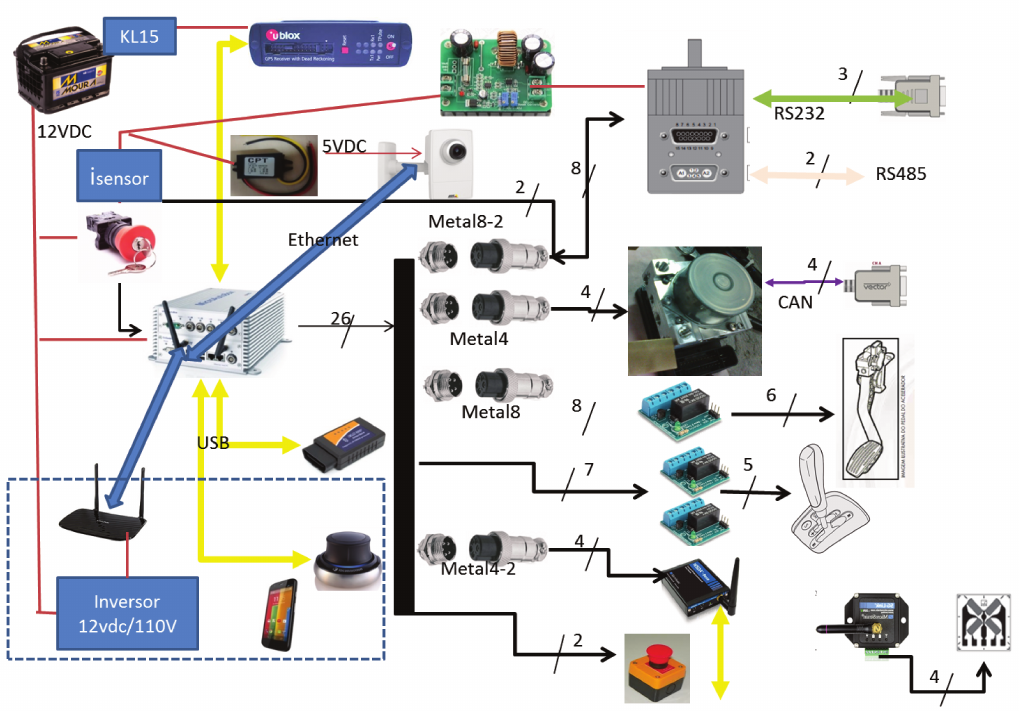
\includegraphics[width=1\linewidth]{img/diagrama_vilma}
				\caption{Diagrama de \textit{hardware} do VILMA01 \cite{bedoya_alise_2016}.}
				\label{fig:diagrama_vilma}
			\end{figure}
			
		\end{column}
		
	\end{columns}
	
	
	
\end{frame}

\begin{frame}{Autoware}
	
	\begin{columns}
		
		\begin{column}{0.3\textwidth}
			
			\begin{figure}[H]
				\centering
				
\includegraphics[width=\linewidth]{autoware_logo}
				\caption{Logomarca do Autoware.}
				\label{fig:autoware_logo}
			\end{figure}
			
		\end{column}
	
\pause
		
		\begin{column}{0.7\textwidth}
			
			\begin{figure}[H]
				\centering
				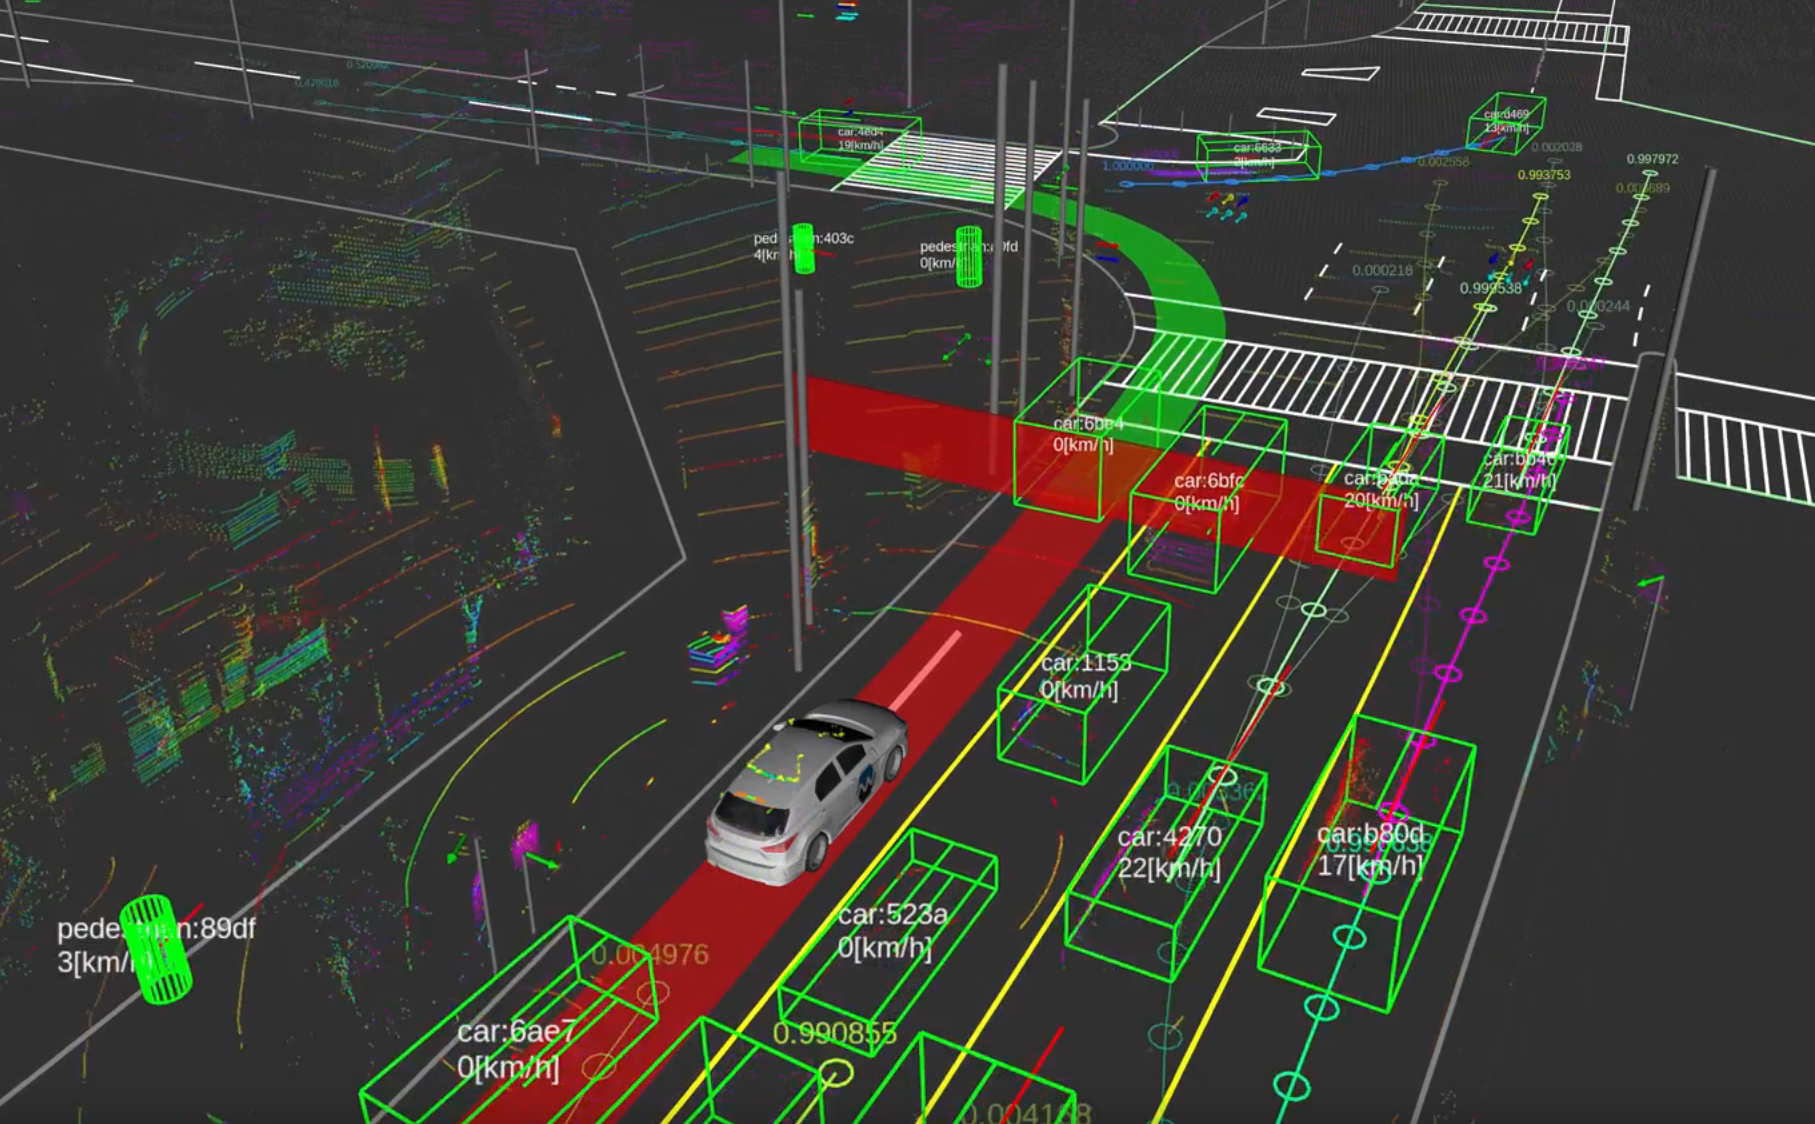
\includegraphics[width=0.9\linewidth]{autoware}
				\caption{Visualização do Autoware em operação \cite{gitautoware}}
				\label{fig:autoware}
			\end{figure}
			
		\end{column}
		
	\end{columns}
	
\end{frame}



\begin{frame}{Arquitetura}
	
	% TODO: \usepackage{graphicx} required
	\begin{figure}
		\centering
		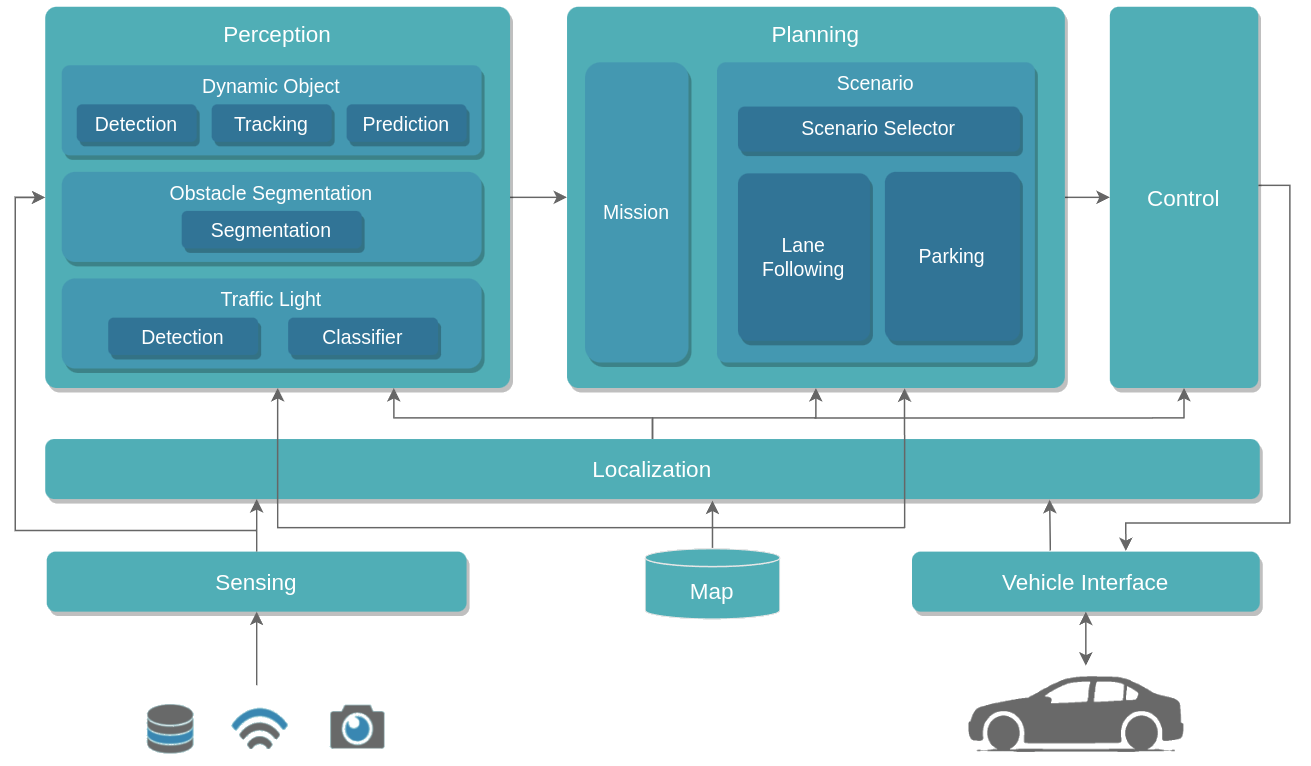
\includegraphics[width=0.8\linewidth]{img/HL_architecture}
		\caption{Arquitetura de alto nível \cite{autowareArchitecture}.}
		\label{fig:hlarchitecture}
	\end{figure}
	
\end{frame}

\section{Proposta}

\begin{frame}{Proposta}
	
	\begin{columns}
		
		\begin{column}{0.35\textwidth}
			
			\begin{block}{}
				
				Trazer o Autoware para dentro do microcontrolador de forma confiável e de fácil implementação.
				
			\end{block}
			
		\end{column}
	
\pause
		
		\begin{column}{0.7\textwidth}
			
			\begin{figure}[H]
				\centering
				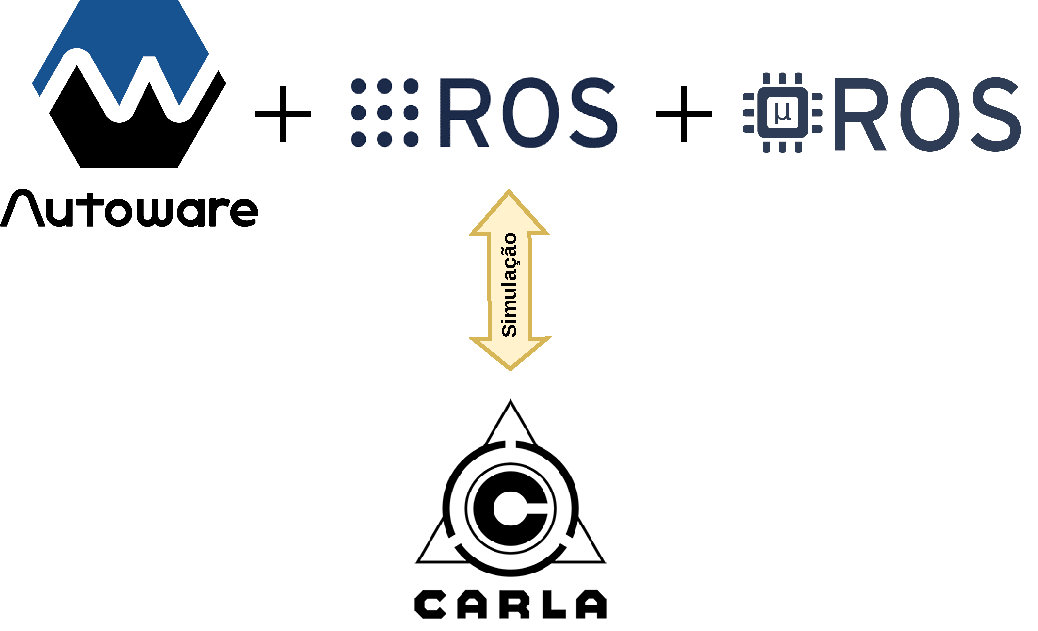
\includegraphics[width=1\linewidth]{logos}
				\caption{Ferramentas para viabilização do projeto.}
				\label{fig:logos}
			\end{figure}
			
		\end{column}
		
	\end{columns}
	
\end{frame}

\begin{frame}{Proposta}
	
	\begin{columns}
		
		\begin{column}{0.6\textwidth}
			
			\begin{figure}[H]
				\centering
				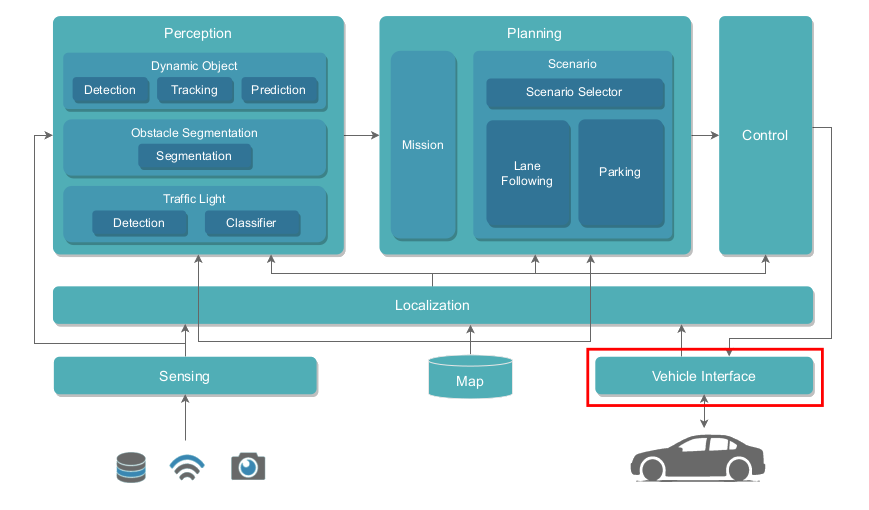
\includegraphics[width=\linewidth]{img/architecture.png}
				\caption{Escopo do projeto na arquitetura Autoware.}
				\label{fig:architecture}
			\end{figure}
			
		\end{column}
		
		\hspace{-0.5cm}
		
\pause
		
		\begin{column}{0.45\textwidth}
			
			\begin{figure}[H]
				\centering
				\includegraphics[width=\linewidth]{img/architecture_HIL}
				\caption{Arquitetura de teste do \textit{hardware}.}
				\label{fig:architecture_HIL}
			\end{figure}
			
		\end{column}
		
	\end{columns}
	
\end{frame}

\begin{frame}{\textit{Vehicle interface}}

% TODO: \usepackage{graphicx} required
\begin{figure}
	\centering
	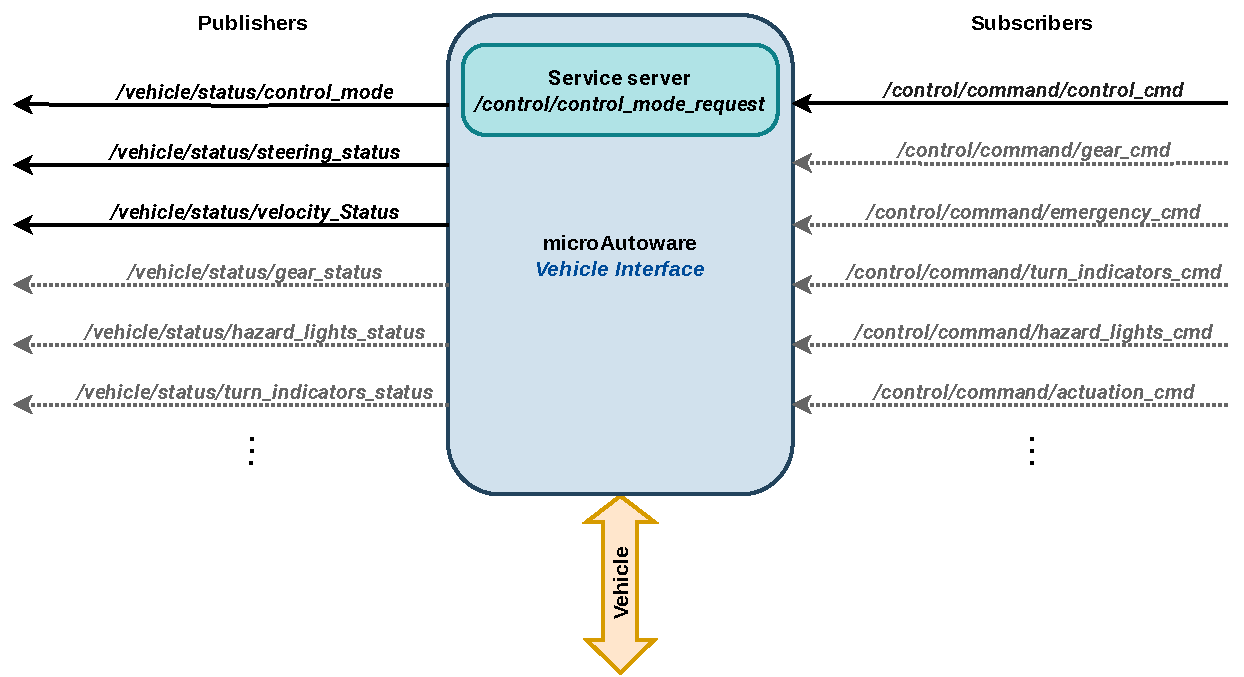
\includegraphics[width=0.8\linewidth]{img/vehicle_interface-topics}
	\caption{Diagrama de tópicos da \textit{vehicle interface}.}
	\label{fig:vehicleinterface-topics}
\end{figure}

\end{frame}

% Vantagens do RTOS

\subsection*{Requisitos}

\begin{frame}{Requisitos}
	
	\begin{columns}
		
		\begin{column}{0.5\textwidth}
			
			\begin{block}{Requisitos funcionais}
				
				\begin{itemize}
					\item \color<2->{FlagGreen}{Comunicação com o Autoware};
					\item \color<2->{FlagGreen}{Controle da aceleração, frenagem e direção do veículo;}
					\item \color<2->{gray}{Controle dos faróis e luzes de sinalização (seta) do veículo;}
					\item \color<2->{FlagGreen}{Teleoperação do veículo por um \textit{joystick} em  \textit{hardware};}
					\item \color<2->{FlagGreen}{Troca do modo de operação por meio da \textit{switch} do \textit{joystick};}
					\item \color<2->{FlagGreen}{Subscrição por meio do micro-ROS em todos os tópicos necessários do Autoware;}
					\item \color<2->{FlagGreen}{Publicação a partir micro-ROS em todos os tópicos necessários do Autoware.}
					\item \color<2->{uscgold}{Comunicação a partir micro-ROS em todos os serviços necessários do Autoware.}
					
				\end{itemize}
				
			\end{block}
			
		\end{column}
		
		\hspace{-0.5cm}
		
\pause
\pause
		
		\begin{column}{0.5\textwidth}
			
			\begin{block}{Requisitos não-funcionais}
				
				\begin{itemize}
					\item \color<4->{FlagGreen}{A \textit{vehicle interface} deve ser construída na forma de um pacote portável para outros microcontroladores STM32;}
					\item \color<4->{FlagGreen}{O interfaceamento com o veículo deve ser intercambiável com diferentes configurações;
					\item \color<4->{FlagGreen}{Deve-se garantir sincronização de \textit{timestamp} entre o Autoware e o microcontrolador;}
					\item O sistema embarcado deve abstraír o veículo como um sistema \textit{Drive-By-Wire} (DBW) para o Autoware.}
				\end{itemize}
				
			\end{block}
			
		\end{column}
		
	\end{columns}
	
\pause
	
\end{frame}

\subsection*{Metodologia}

\begin{frame}{Modelo de desenvolvimento}
	
	\begin{columns}
		
		\begin{column}{0.4\textwidth}
			
			\begin{block}{Modelo V}
				
				\begin{itemize}
					\item Realização e validação de cada etapa do projeto em paralelo.
					
				\end{itemize}
				
			\end{block}
			
		\end{column}
		
		\begin{column}{0.7\textwidth}
			
			
			% TODO: \usepackage{graphicx} required
			\begin{figure}
				\centering
				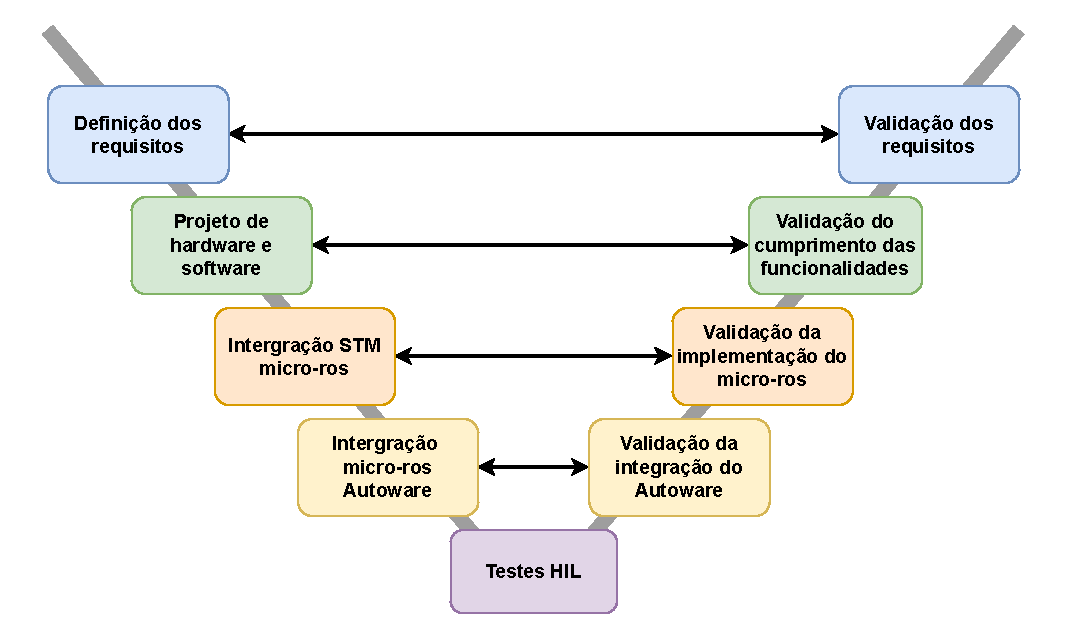
\includegraphics[width=\linewidth]{img/modelo-v}
				\caption{Modelo de execução das atividades do projeto.}
				\label{fig:modelo-v}
			\end{figure}
			
		\end{column}
		
	\end{columns}
	
\end{frame}

\section{Desenvolvimento}

\subsection*{Diagrama de blocos}

\begin{frame}{Diagrama de blocos}
	
	\begin{figure}[H]
		\centering
		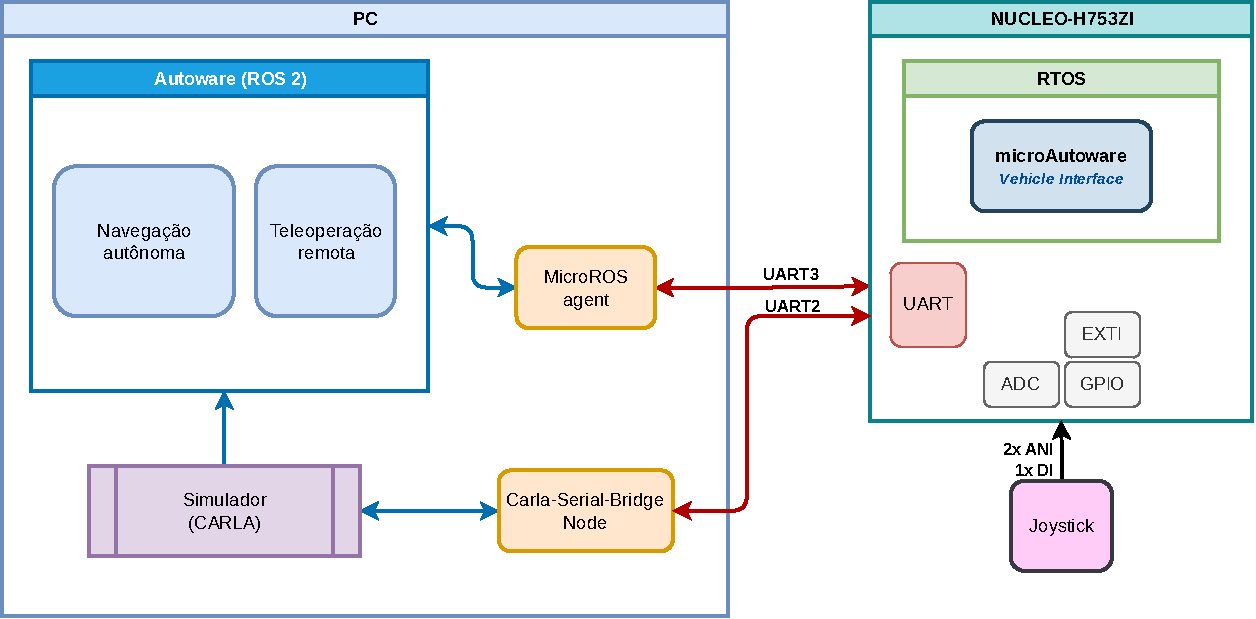
\includegraphics[width=0.9\linewidth]{block_diagram}
		\caption{Diagrama de blocos atualizado.}
		\label{fig:block_diagram}
	\end{figure}
	
\end{frame}

\subsection*{Esquemático}

\begin{frame}{Esquemático}
	
	
	\begin{figure}
		\centering
		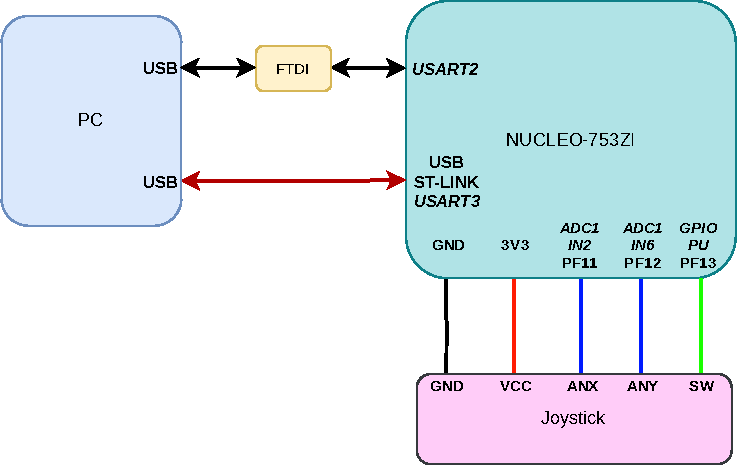
\includegraphics[width=0.75\linewidth]{img/esquematico.pdf}
		\caption{Esquemático de ligações elétricas.}
		\label{fig:esquematico}
	\end{figure}
	
\end{frame}

\subsection*{\textit{Joystick}}

\begin{frame}{\textit{Joystick}}
	
	\begin{columns}
		
		\begin{column}{0.5\textwidth}
			
			\begin{figure}[H]
				\centering
				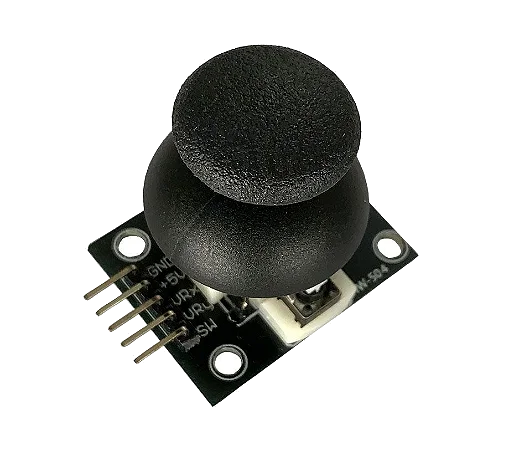
\includegraphics[width=0.75\linewidth]{joystick}
				\caption{caption}
				\label{fig:label}
			\end{figure}
			
		\end{column}
		
		\begin{column}{0.5\textwidth}
			
			\begin{block}{}
				
				\textbf{Eixos $x$ e $y$}
				\begin{itemize}
					\item ADC de 16 bits \textit{multi-channel};
					\item Leitura contínua por DMA.					
				\end{itemize}
			
				\textbf{Botão}
				\begin{itemize}
					\item GPIO em modo \textit{pull-up};
					\item Interrupção EXTI.
					
				\end{itemize}
			
				
			\end{block}
			
		\end{column}
		
	\end{columns}
	
\end{frame}

\begin{frame}{Processamento de sinais}
	
	\begin{columns}
		
		\begin{column}{0.5\textwidth}
			
			
			% TODO: \usepackage{graphicx} required
			\begin{figure}
				\centering
				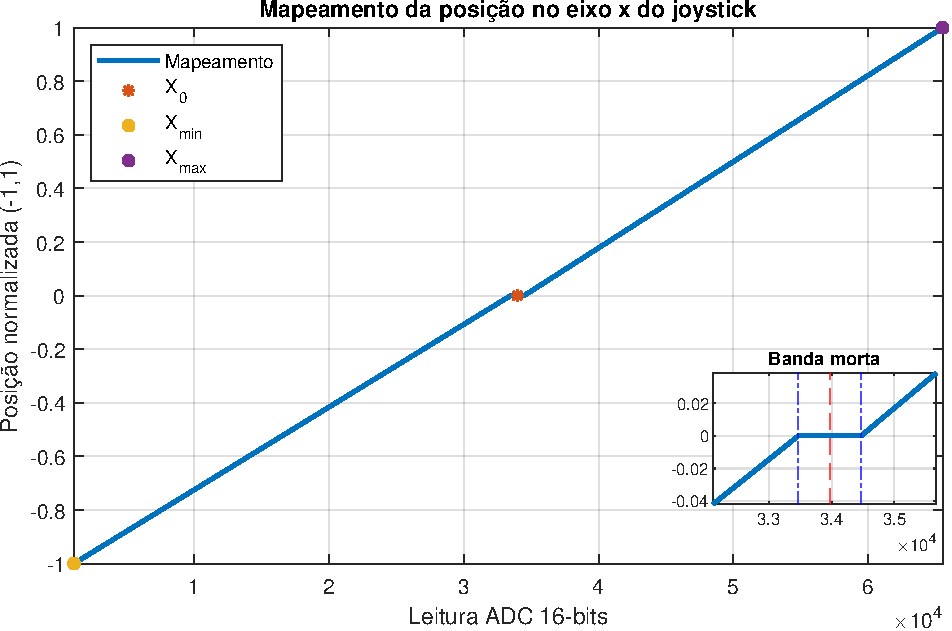
\includegraphics[width=1.1\linewidth]{plot_joy_x_axis.pdf}
				\caption{Mapeamento da posição normalizada do \textit{joystick} de acordo com a leitura analógia do ADC.}
				\label{fig:plotjoyxaxis}
			\end{figure}
			
		\end{column}
	
\pause
		
		\begin{column}{0.6\textwidth}
			
			\begin{equation}\label{eq:joy}
				p(v) = \begin{dcases}
					0\vphantom{\frac{0}{0}}, &\text{se } - B \le v - V_0 \le B \\
					\frac{v - V_0 - B}{V_{max} - V_0 - B}, &\text{se } v > V_0 + B \\
					\frac{v - V_0 + B}{V_0 - V_{min} - B}, &\text{se } v < V_0 - B 
				\end{dcases}
			\end{equation}
			
		\end{column}
		
	\end{columns}
	
\end{frame}

\begin{frame}{Estados do sistema}
	
	
	\begin{figure}[H]
		\centering
		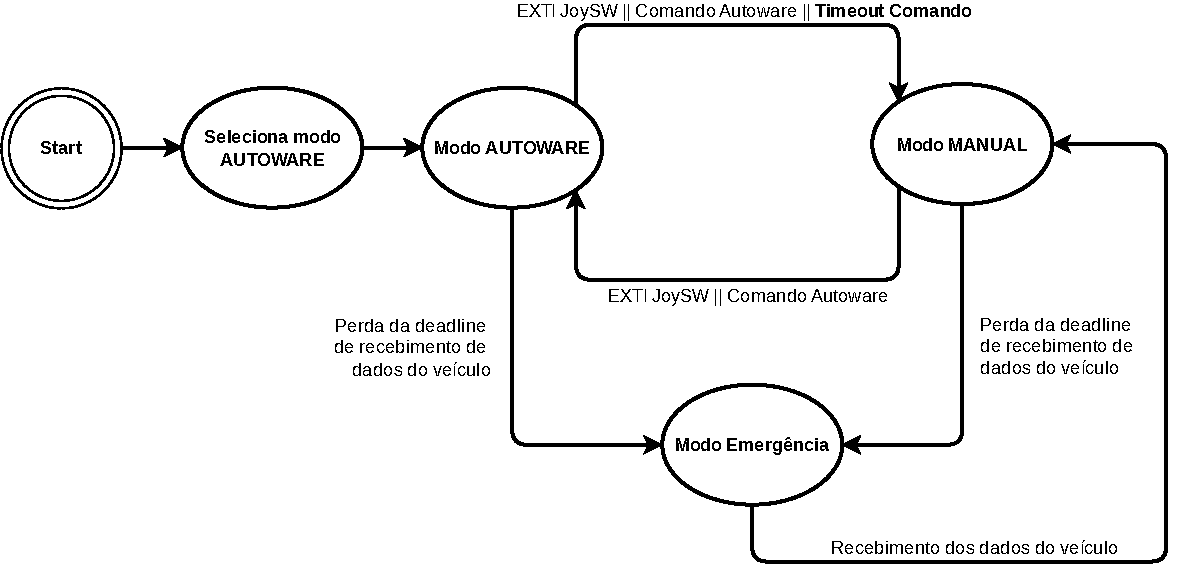
\includegraphics[width = \textwidth]{img/maquinadeestados}
		\caption{Máquina de estados do sistema.}
		\label{fig:maquinadeestados}
	\end{figure}
	
	
\end{frame}

\subsection*{Tarefas}

\begin{frame}{Diagrama de tarefas}
	
	\begin{figure}[H]
		\centering
		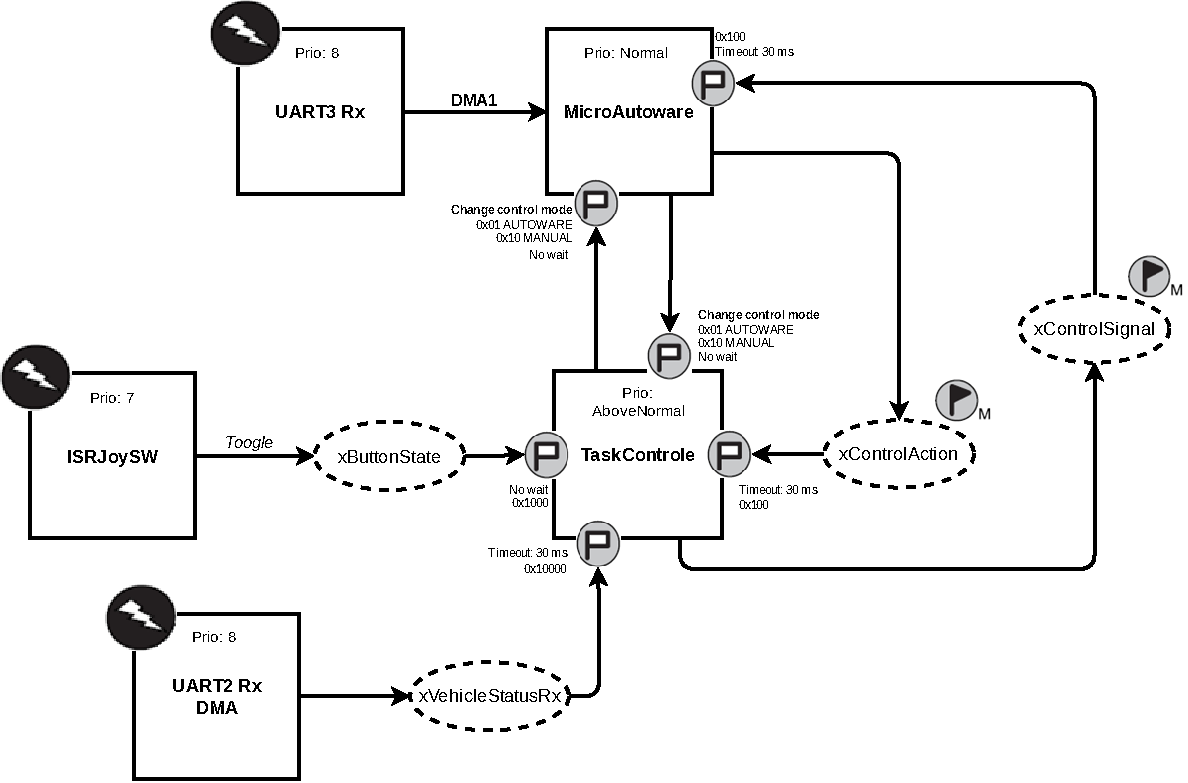
\includegraphics[width=0.75\linewidth]{system_diagram}
		\caption{Diagrama de tarefas atualizado.}
		\label{fig:system_diagram}
	\end{figure}
	
\end{frame}

\begin{frame}{Comunicação e sincronização de tarefas}
	
	\begin{columns}
		
		\begin{column}{0.5\textwidth}
			
			\begin{block}{Comunicação}
				
				\begin{itemize}
					\item Variáveis globais protegidas por mutex;
					\item \textit{ThreadFlags}.					
				\end{itemize}
				
			\end{block}
			
		\end{column}
		
		\begin{column}{0.5\textwidth}
			
			\begin{block}{Sincronização}
				
				\begin{itemize}
					\item \textit{ThreadFlags}.	
					
				\end{itemize}		
				
			\end{block}
			
		\end{column}
		
	\end{columns}
	
\end{frame}


\subsection*{Comunicação}

\begin{frame}{Configuração dos módulos UART}
	
	\begin{columns}
		
		\begin{column}{0.5\textwidth}
			
			\begin{block}{UART2}
				
				Comunicação com o simulador.
				\begin{itemize}
					\item \textbf{\textit{Baudrate}:} 921600 bps
					\item \textbf{Modo de leitura:} DMA circular;
					\item \textbf{Modo de escrita:} DMA única;
					\item \textbf{Interface física:} ST-LINK.
				\end{itemize}
				
			\end{block}
			
		\end{column}
	
\pause
		
		\begin{column}{0.5\textwidth}
			
			\begin{block}{UART3}
				
				Comunicação com o Autoware.
				\begin{itemize}
					\item \textbf{\textit{Baudrate}:} 921600 bps
					\item \textbf{Modo de leitura:} DMA única;
					\item \textbf{Modo de escrita:} DMA única;
					\item \textbf{Interface física:} Módulo FTDI			
				\end{itemize}
				
			\end{block}
			
		\end{column}
		
	\end{columns}
	
\end{frame}

\begin{frame}{Comunicação com o simulador}
	
	\begin{columns}
		
		\begin{column}{0.435\textwidth}
			
			\begin{block}{Sistema embarcado $\longrightarrow$ CARLA}
				
				\begin{itemize}
					\item \texttt{float fSteeringAngle;}
					\item \texttt{float fSteeringVelocity;}
					\item \texttt{float fSpeed;}
					\item \texttt{float fAcceleration;}
					\item \texttt{float fJerk;}	
					\item \texttt{unsigned char ucControlMode;}					
				\end{itemize}
				
			\end{block}
			
		\end{column}
	
\pause
		
		\begin{column}{0.435\textwidth}
			
			\begin{block}{CARLA $\longrightarrow$ Sistema embarcado }
				
				\begin{itemize}
					\item \texttt{float fLongSpeed;}
					\item \texttt{float fLatSpeed;}
					\item \texttt{float fHeadingRate;}
					\item \texttt{float fSteeringStatus;}
					
				\end{itemize}
				
				
				
			\end{block}
			
		\end{column}
		
	\end{columns}

\pause
	
	\begin{block}{}
		
		\textbf{Padrão de Mensagem:} Sistema embarcado $\longrightarrow$ CARLA
		
		\begin{itemize}
			\item \textbf{\#S}\texttt{\%c\%c\%c\%c}\textbf{W}\texttt{\%c\%c\%c\%c}\textbf{V}\texttt{\%c\%c\%c\%c}\textbf{A}\texttt{\%c\%c\%c\%c}\textbf{J}\texttt{\%c\%c\%c\%c}\textbf{M}\texttt{\%c}\textbf{\$}
			\item 30 bytes
			
		\end{itemize}
		
		\textbf{Padro de Mensagem:} CARLA $\longrightarrow$ Sistema embarcado
		\begin{itemize}
			\item \textbf{\#A}\texttt{\%c\%c\%c\%c}\textbf{B}\texttt{\%c\%c\%c\%c}\textbf{C}\texttt{\%c\%c\%c\%c}\textbf{D}\texttt{\%c\%c\%c\%c}\textbf{\$}
			\item 22 bytes
			
		\end{itemize}
		
	\end{block}
	
\end{frame}

\begin{frame}{Máquinas de estados de comunicação}
	
	\begin{figure}[H]
		\centering
		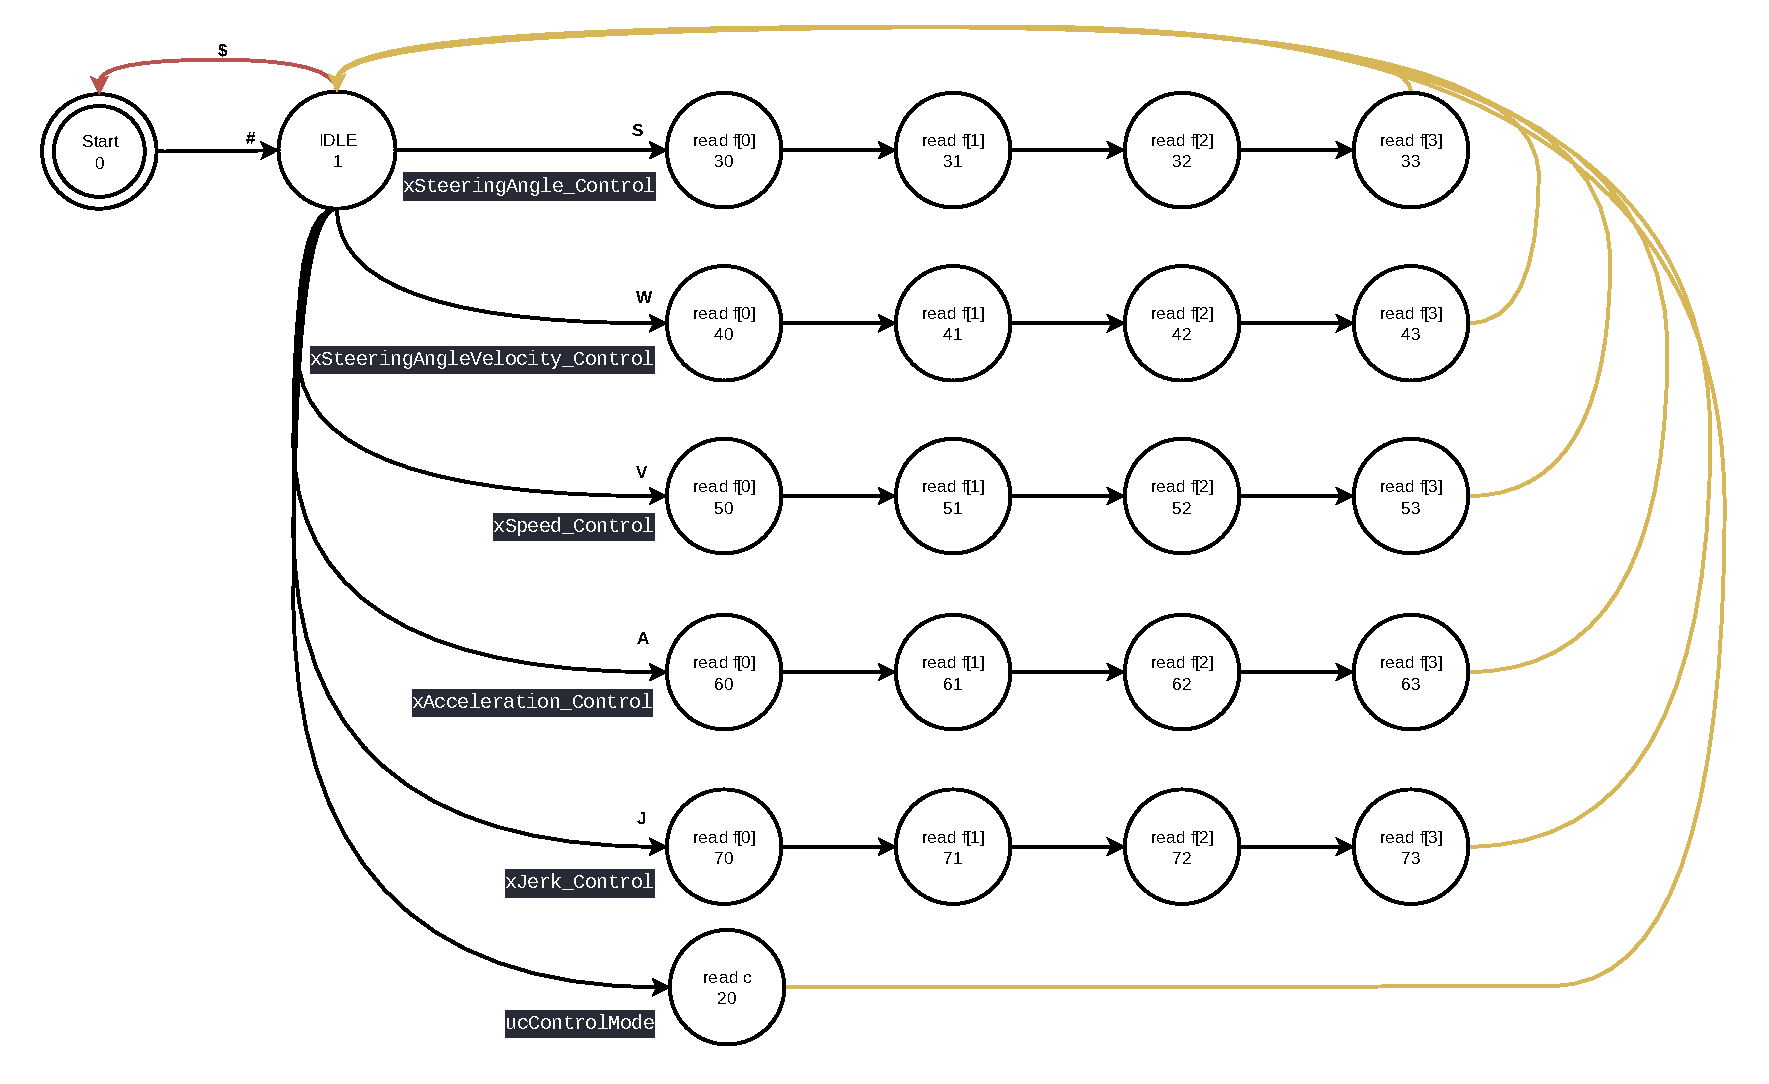
\includegraphics[width=0.8\linewidth]{sm_uc_2_carla}
		\caption{Maquina de estados da comunicação sistema embarcado $\longrightarrow$ CARLA (\texttt{CarlaSerialBridgeNode}).}
		\label{fig:sm_uc_2_carla}
	\end{figure}
	
\end{frame}

\begin{frame}{Máquinas de estados de comunicação}
	
	\begin{figure}[H]
		\centering
		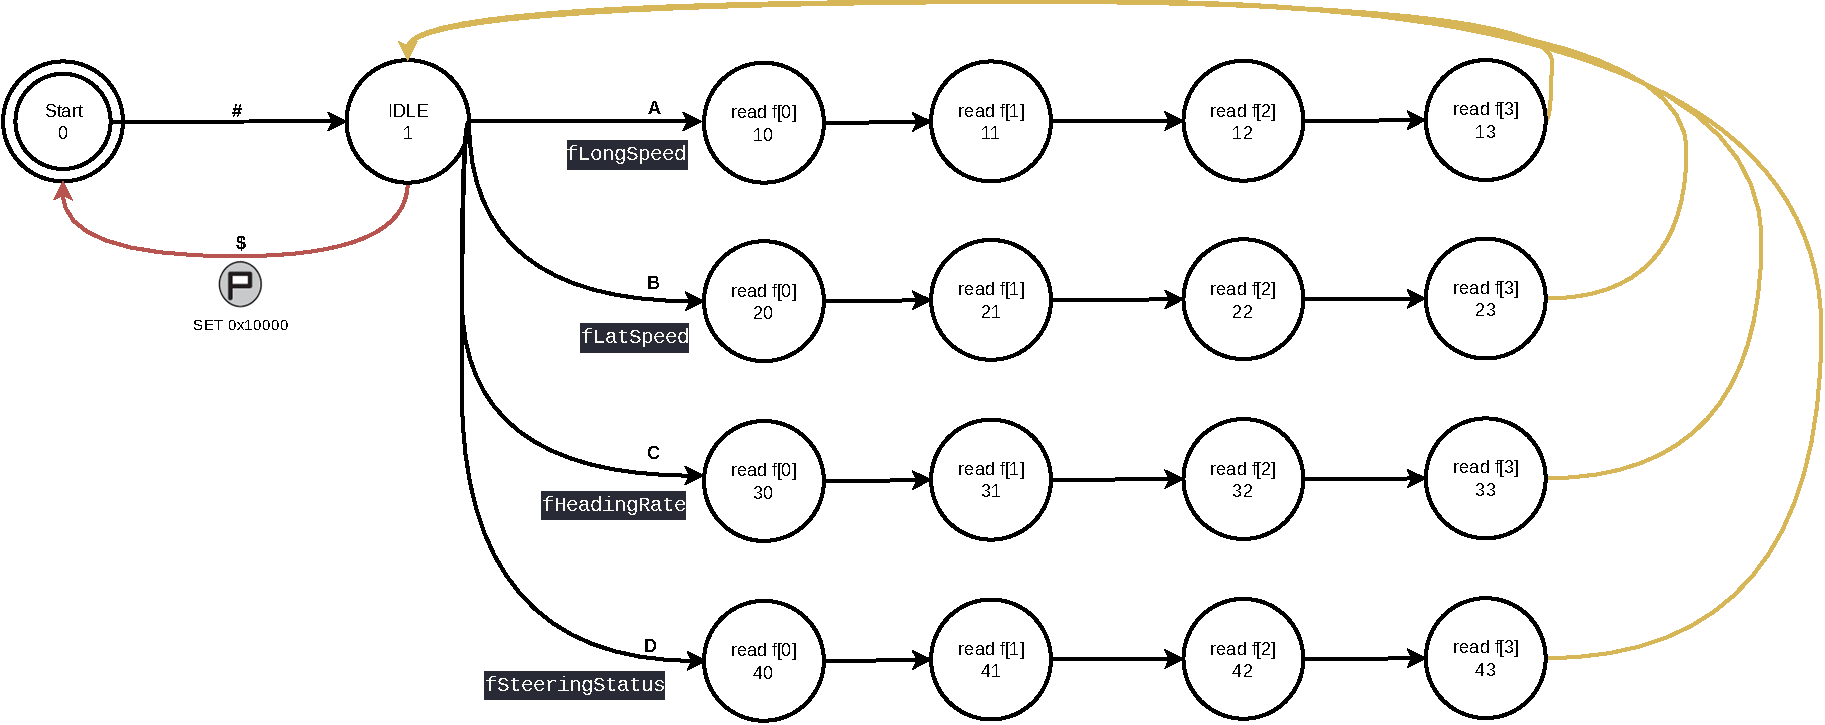
\includegraphics[width=\linewidth]{sm_carla_2_uc}
		\caption{Maquina de estados da comunicação CARLA $\longrightarrow$ sistema embarcado (\texttt{HAL\_UART\_RxCpltCallback()}).}
		\label{fig:sm_carla_2_uc}
	\end{figure}
	
\end{frame}


\subsection*{Diagrama de nós e tópicos}




\section{Resultados}

\subsection*{Inicialização do Autoware}

\begin{frame}{Inicialização do Autoware}
	
	\begin{figure}[H]
		\centering
		\movie[width=0.85\textwidth,height=0.478\textwidth,poster,autostart,loop]{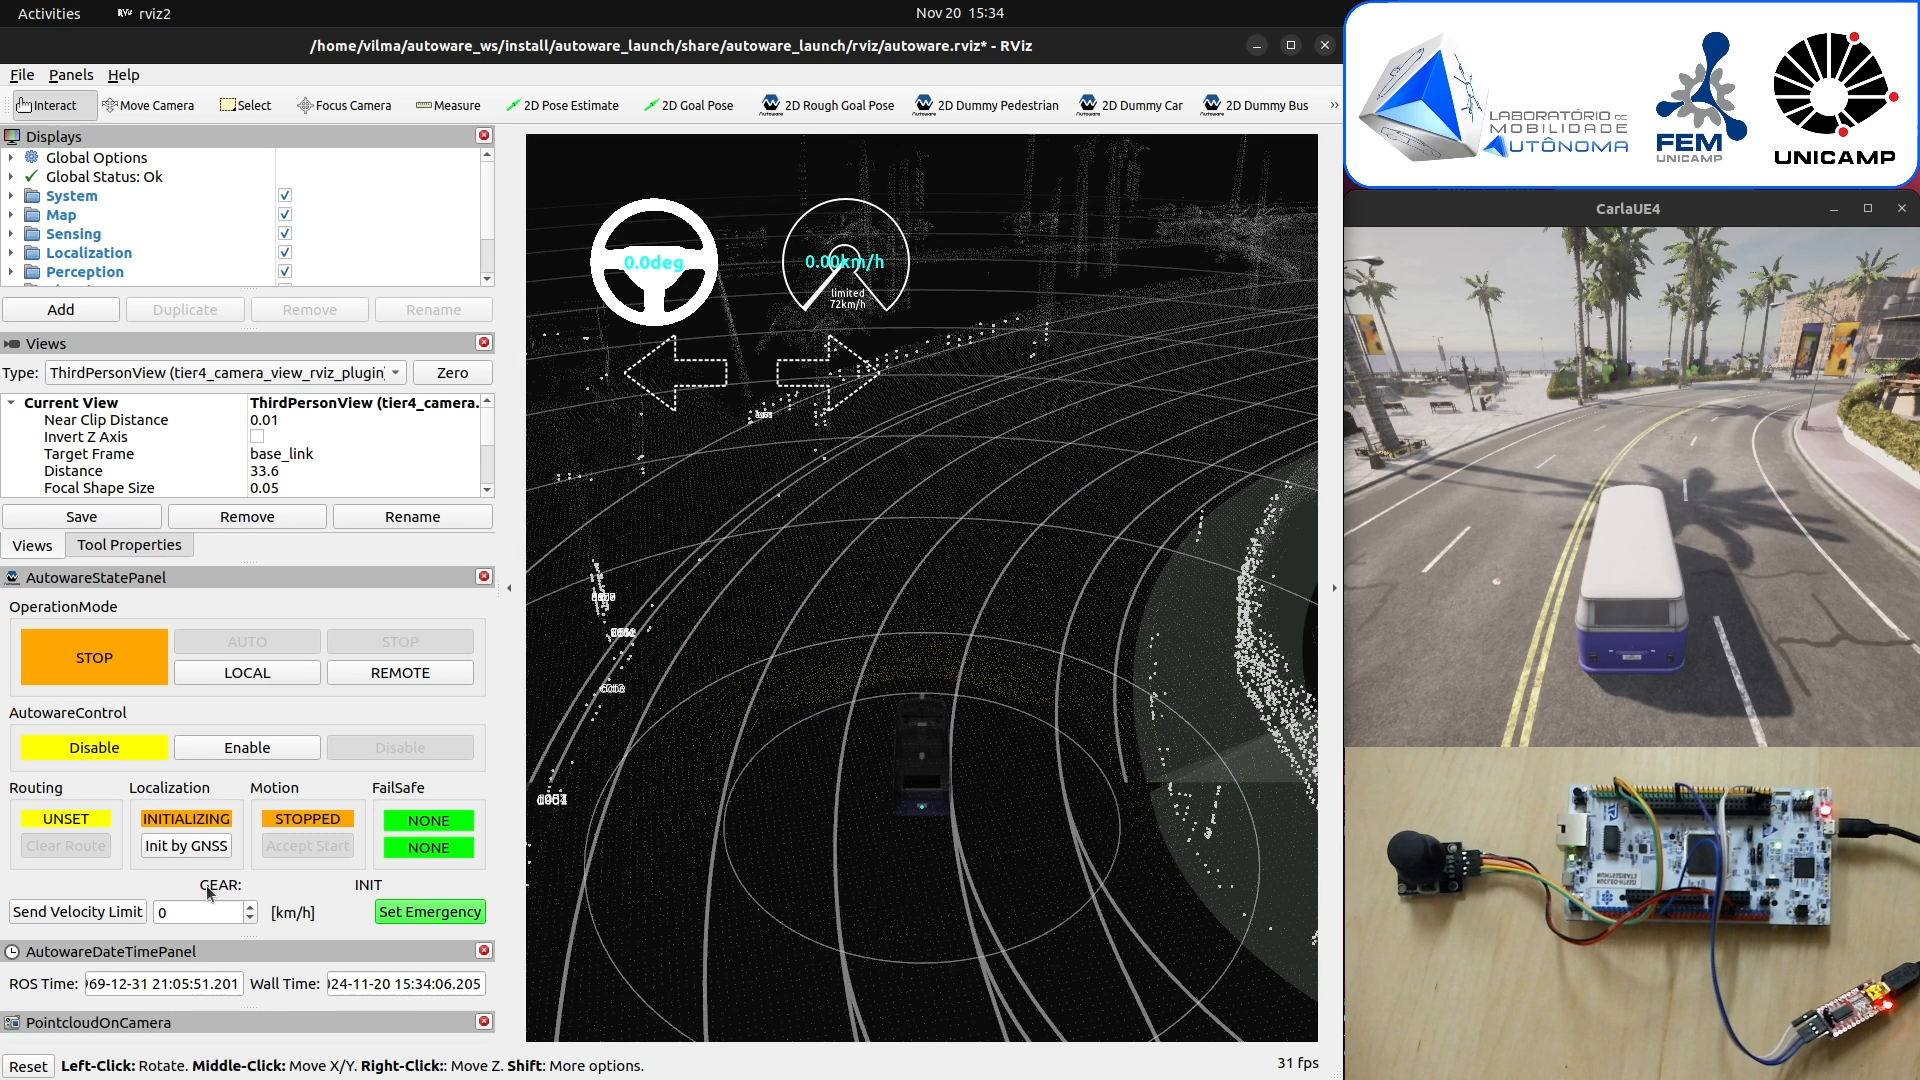
\includegraphics[width=0.85\linewidth]{microautoware_testing_initialization}}{microautoware_testing_initialization.mp4}
		\caption{Inicialização.}
		\label{fig:microautoware_testing_initialization}
	\end{figure}
	
\end{frame}

\subsection*{Controle manual}

\begin{frame}{Controle manual}

\begin{figure}[H]
	\centering
	\movie[width=0.85\textwidth,height=0.478\textwidth,poster,autostart,loop]{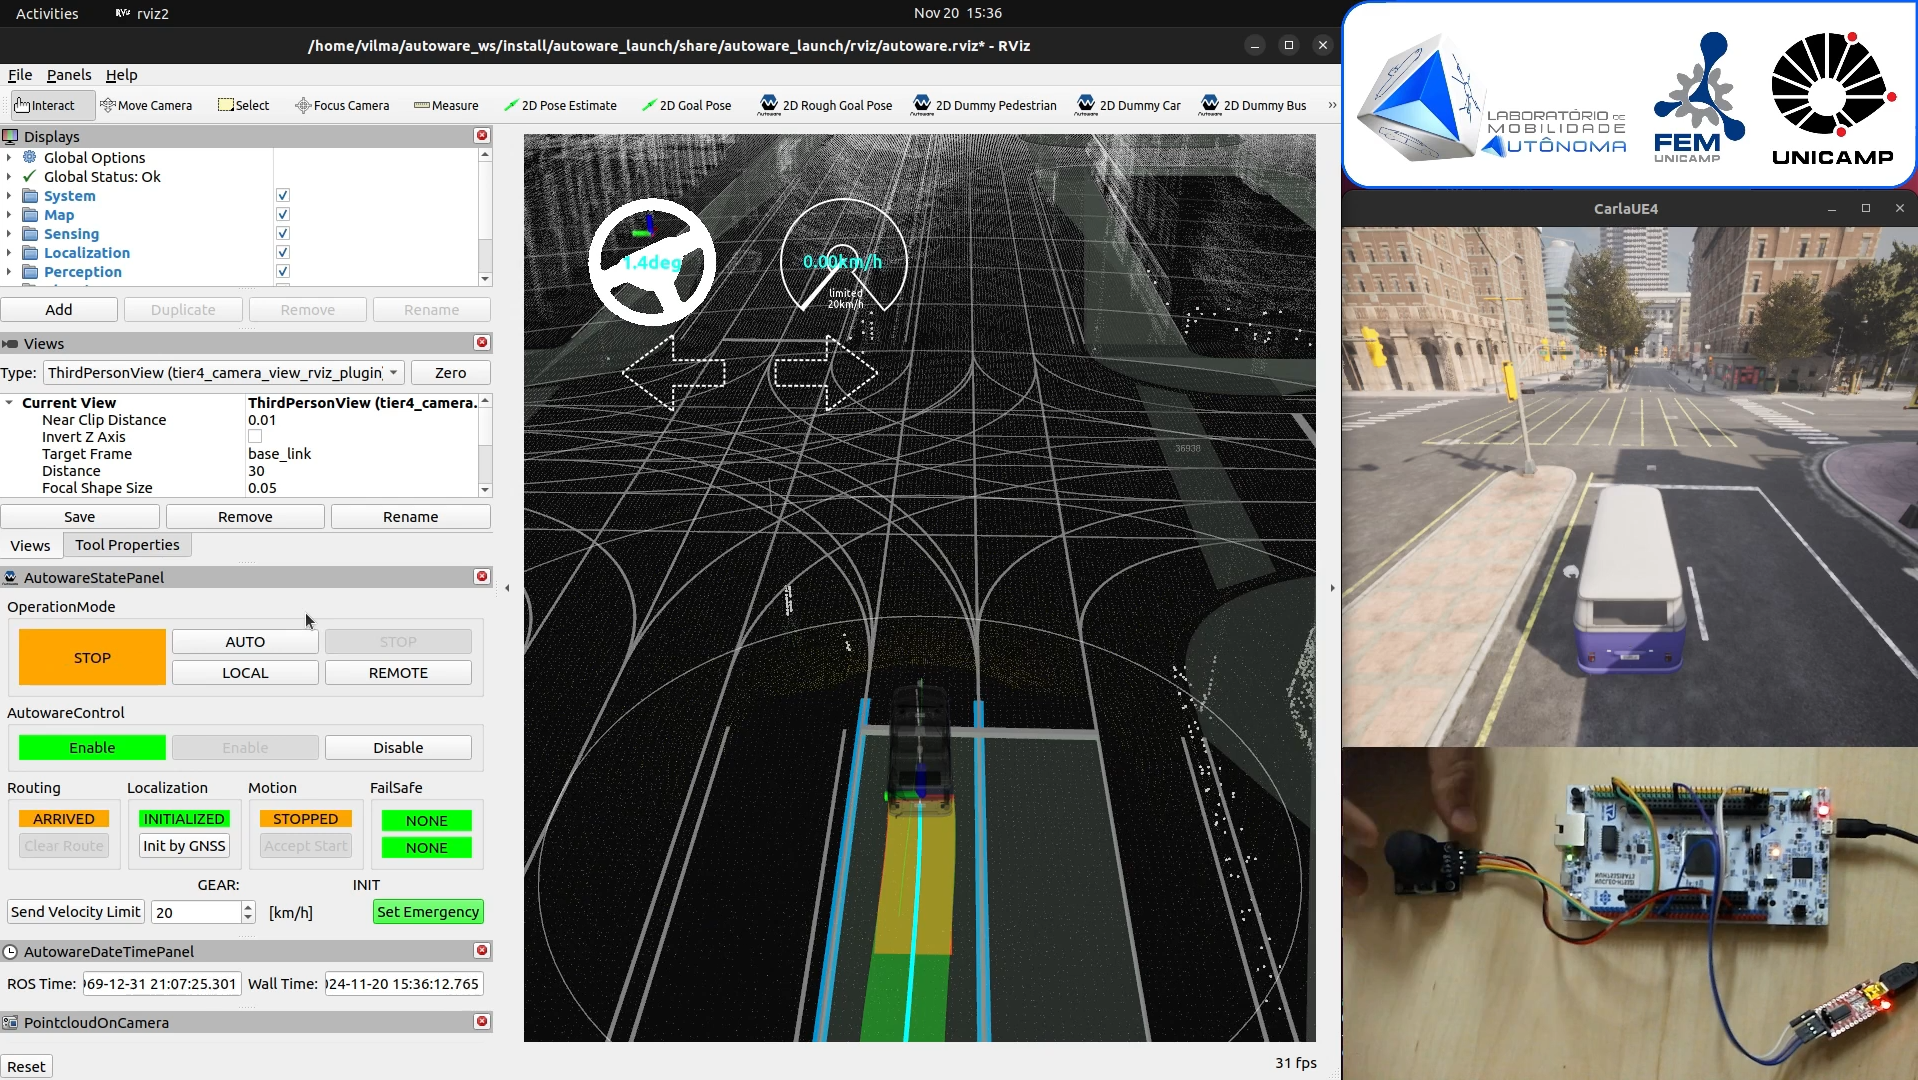
\includegraphics[width=0.85\linewidth]{microautoware_testing_manual_mode}}{microautoware_testing_manual_mode.mp4}
	\caption{Controle manual.}
	\label{fig:microautoware_testing_manual_mode}
\end{figure}

\end{frame}

\subsection*{Controle autônomo}

\begin{frame}{Controle autônomo}
	
	\begin{figure}[H]
		\centering
		\movie[width=0.85\textwidth,height=0.478\textwidth,poster,autostart,loop]{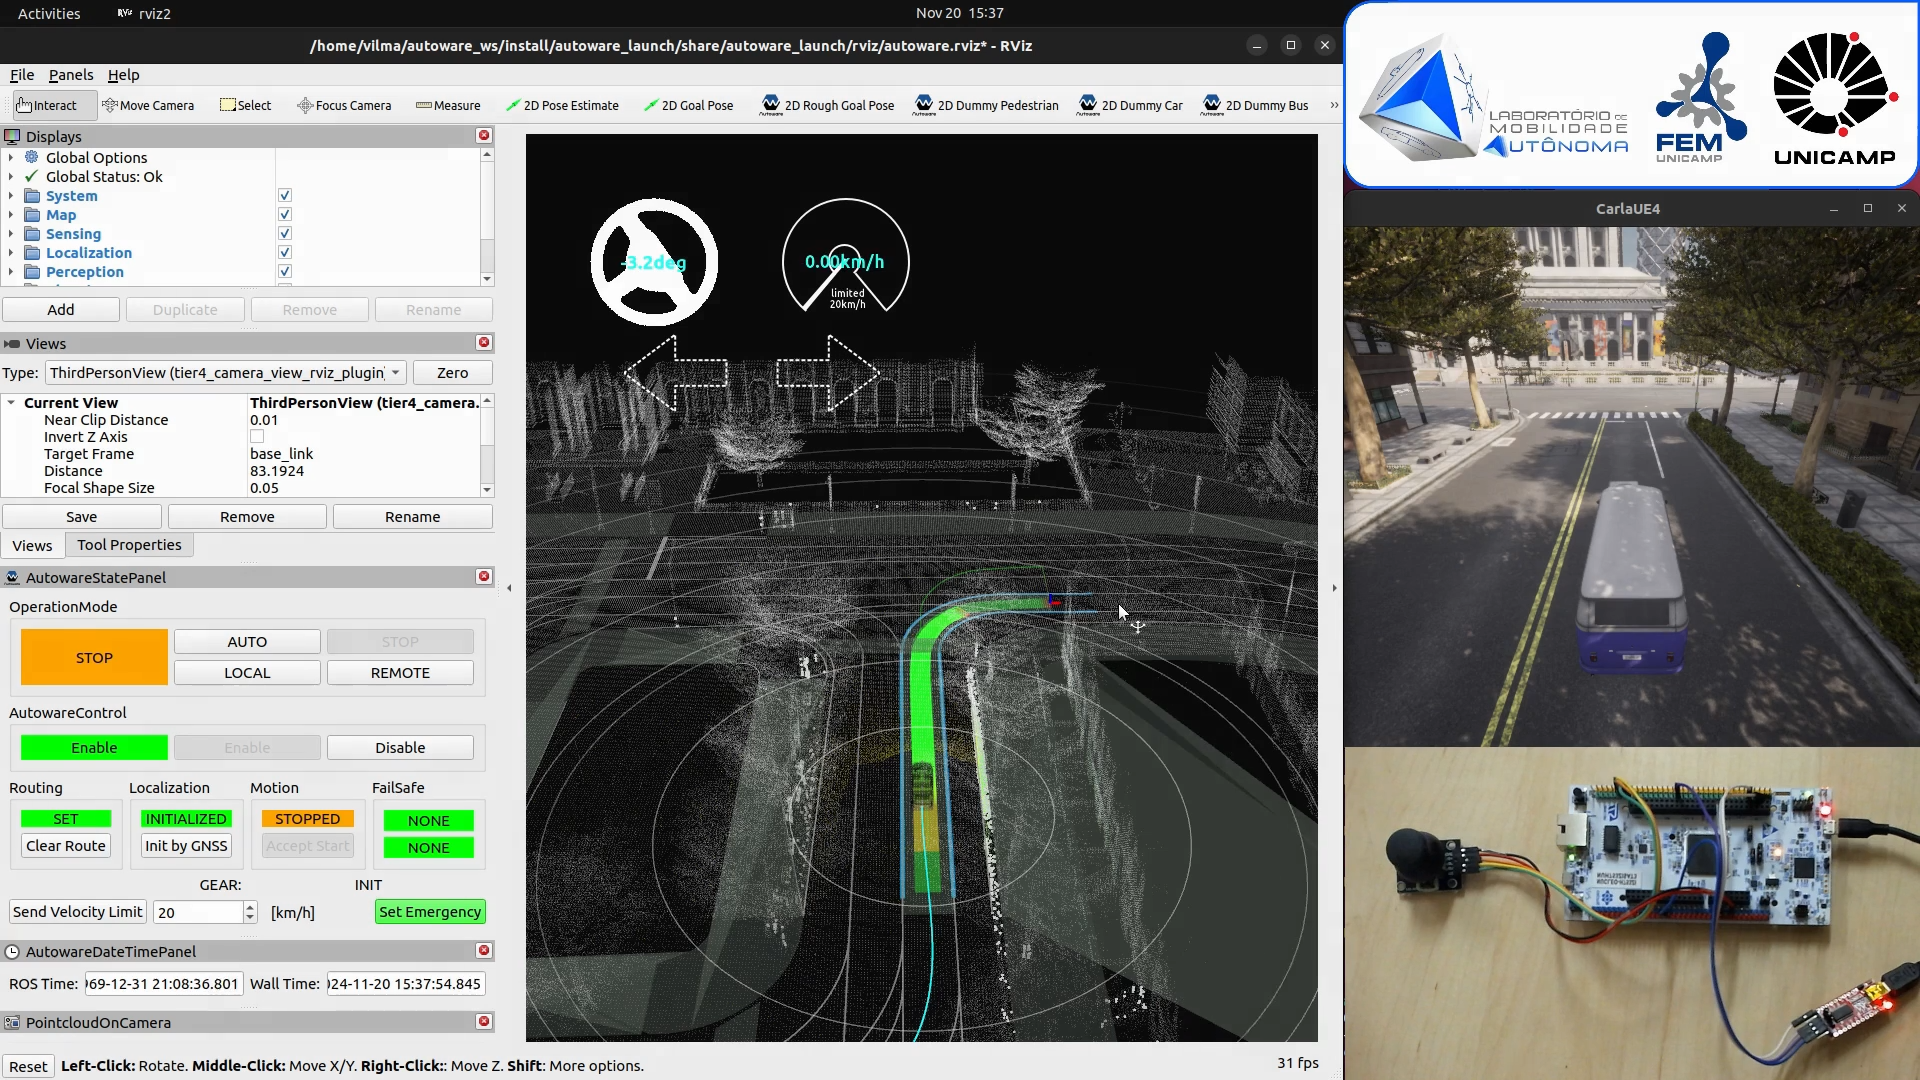
\includegraphics[width=0.85\linewidth]{microautoware_testing_autonomous_mode}}{microautoware_testing_autonomous_mode.mp4}
		\caption{Controle autonomo.}
		\label{fig:microautoware_testing_autonomous_mode}
	\end{figure}
	
\end{frame}

\subsection*{Troca de modo de controle}

\begin{frame}{Troca de modo de controle -- \textit{Joystick}}
	
	\begin{figure}[H]
		\centering
		\movie[width=0.85\textwidth,height=0.478\textwidth,poster,autostart,loop]{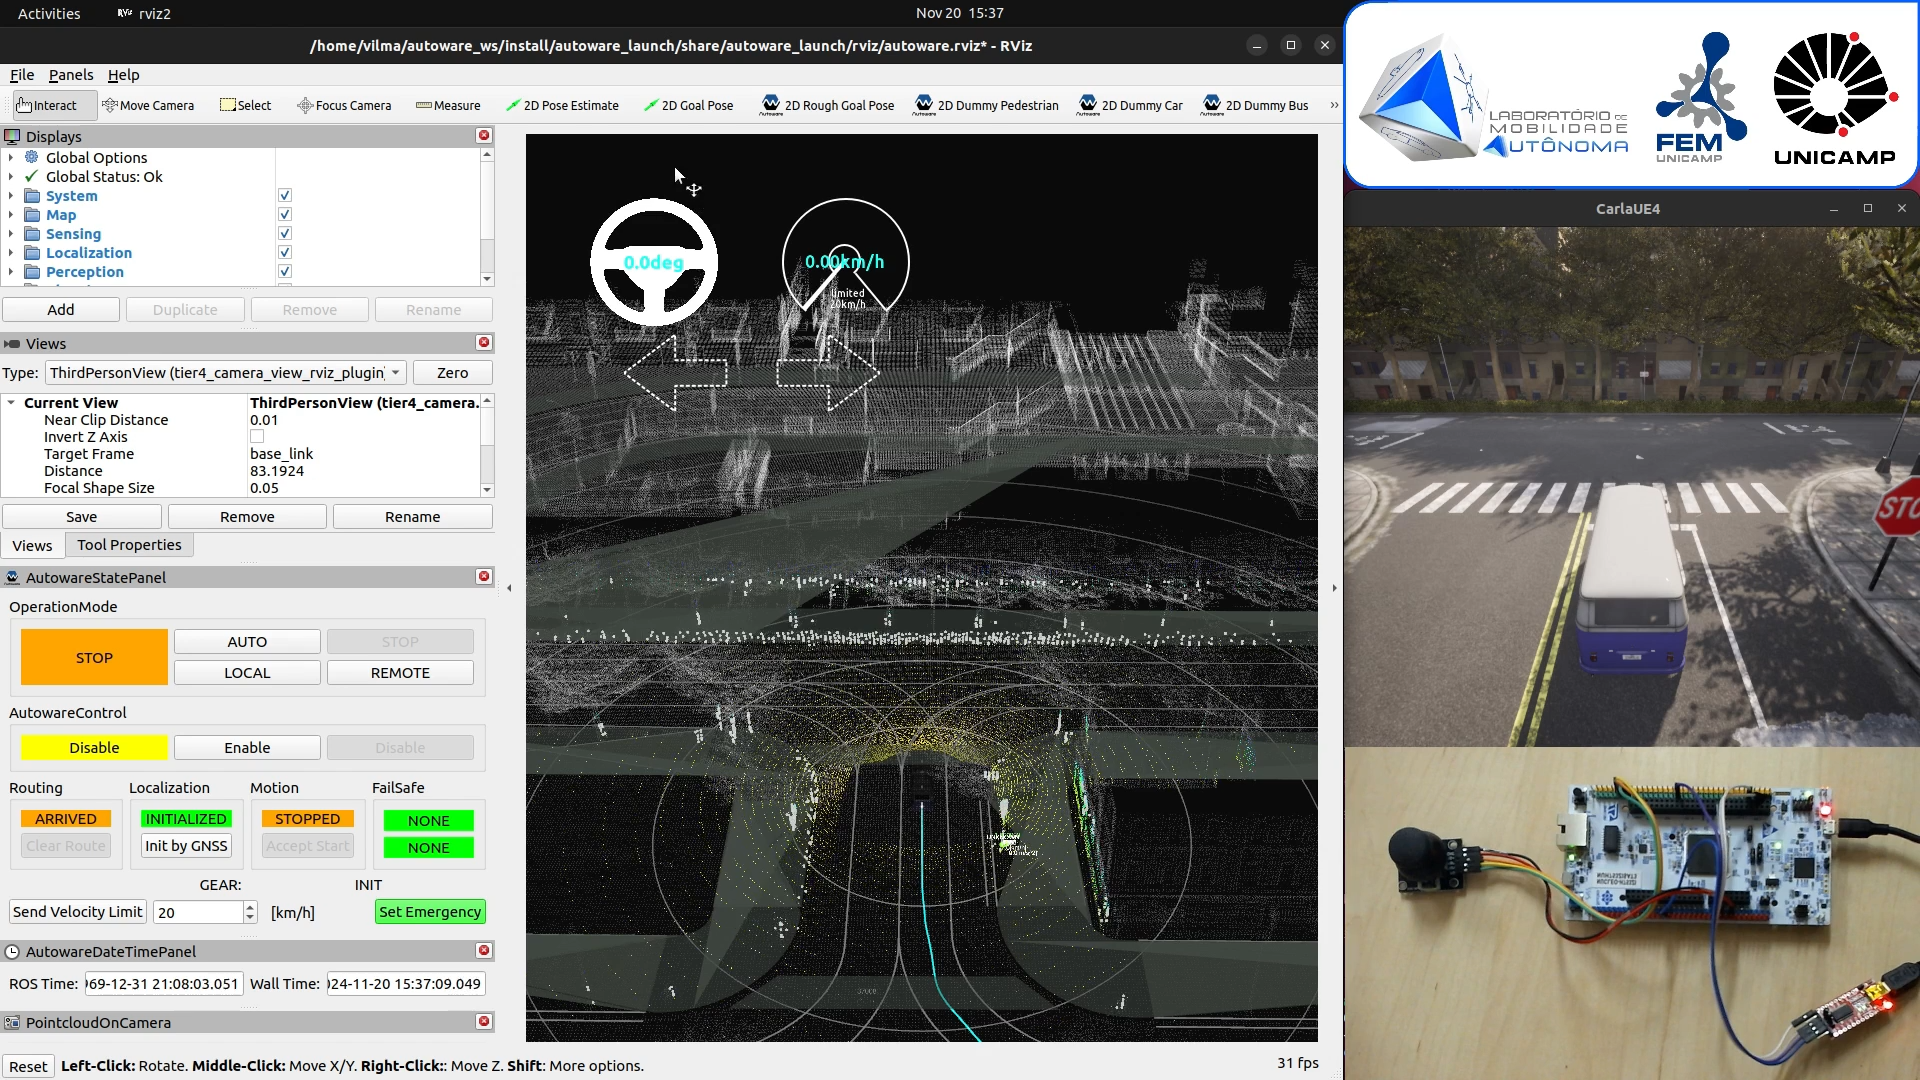
\includegraphics[width=0.85\linewidth]{microautoware_testing_autonomous_w_control_mode_change}}{microautoware_testing_autonomous_w_control_mode_change.mp4}
		\caption{Troca do modo de controle pelo \textit{joystick}.}
		\label{fig:microautoware_testing_autonomous_w_control_mode_change}
	\end{figure}
		
\end{frame}

\begin{frame}{Troca de modo de controle -- Autoware}
	
	\begin{figure}[H]
		\centering
		\movie[width=0.85\textwidth,height=0.478\textwidth,poster,autostart,loop]{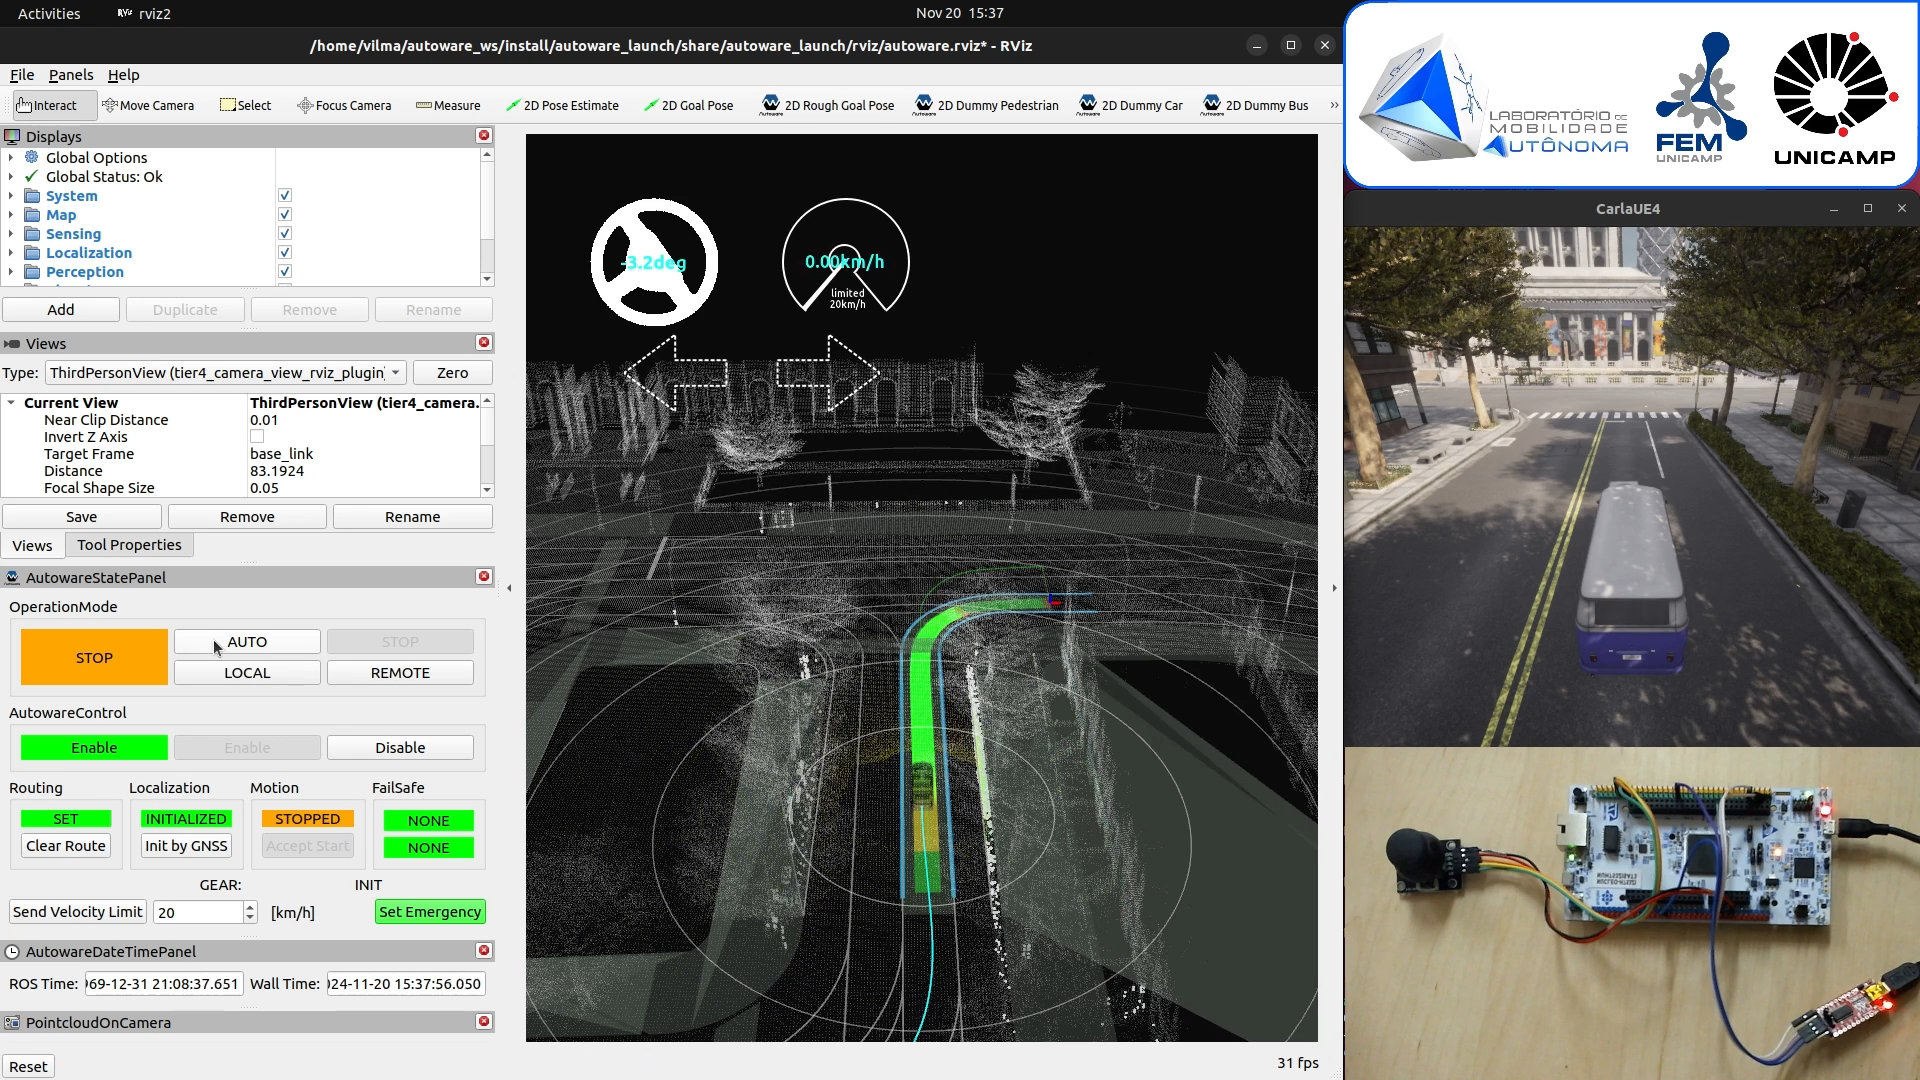
\includegraphics[width=0.85\linewidth]{microautoware_testing_autonomous_w_manual_mode_take_up}}{microautoware_testing_autonomous_w_manual_mode_take_up.mp4}
		\caption{Tomada de condução para modo manual e troca de modo de operação pelo Autoware.}
		\label{fig:microautoware_testing_autonomous_w_manual_mode_take_up}
	\end{figure}
\end{frame}

\subsection*{Modo de emergência}

\begin{frame}{Modo de emergência}
	
	Perder autoware
	
	Perder carla (RX)
	
\end{frame}

\subsection*{Repositório}

\begin{frame}{Repositório no GitHub}
	
	
	
\end{frame}


\section{Conclusão}

\subsection*{Problemas encontrados}

\subsection*{Trabalhos futuros}


\begin{frame}{Cronograma}
	
	
	\begin{table}
		\centering
		\small{
			\begin{tabular}{|b|b|b|b|b|b|b|b|b|b|}
				\hline
				\textbf{Atividade/Semana} & 1 \cellcolor{lightgray} & \textbf{2} \cellcolor{lightgray} & 3 \cellcolor{lightgray} & \textbf{4} \cellcolor{lightgray} & 5 \cellcolor{lightgray} & 6 \cellcolor{lightgray} & \textbf{7} \cellcolor{lightgray} & 8\cellcolor{lightgray} & \textbf{9} \cellcolor{lightgray}\\
				\hline
				Proposta do projeto  & \cellcolor{unifeiblue} &  &  &  &  &  &  &  &  \\
				\hline
				Projeto de \textit{hardware} e \textit{software}  &  & \cellcolor{unifeiblue} & \cellcolor{unifeiblue} &  &  &  &  &  &  \\
				\hline
				Integração do STM com o micro-ROS  &  & \cellcolor{unifeiblue} &  &  &  &  &  &  &  \\
				\hline
				Integração do micro-ROS com o Autoware  &  &  & \cellcolor{unifeiblue} & \cellcolor{unifeiblue} & \cellcolor{unifeiblue} &  &  &  &  \\
				\hline
				Implementação das tarefas do sistema embarcado  &  &  &  & \cellcolor{unifeiblue} & \cellcolor{unifeiblue} & \cellcolor{unifeiblue} & \cellcolor{unifeiblue} &  &  \\
				\hline
				Construção do ambiente de testes  &  &  &  &  & \cellcolor{unifeiblue} & \cellcolor{unifeiblue} & \cellcolor{unifeiblue} &  &  \\
				\hline
				Realização dos testes  &  &  &  &  &  &  & \cellcolor{unifeiblue} & \cellcolor{unifeiblue} & \cellcolor{unifeiblue} \\
				\hline
				Escrita do relatório  &   & \cellcolor{unifeiblue} & \cellcolor{unifeiblue} & \cellcolor{unifeiblue} & \cellcolor{unifeiblue} & \cellcolor{unifeiblue} & \cellcolor{unifeiblue} & \cellcolor{unifeiblue} & \cellcolor{unifeiblue} \\
				\hline
			\end{tabular}
		}
		\caption{Cronograma de atividades.}
		\label{tab:crono}
	\end{table}
	
	\begin{itemize}
		\small
		\color{gray}{\item \textbf{Semana 2:} Apresentação Etapa 1
		\item \textbf{Semana 4:} Apresentação Etapa 2
		\item \textbf{Semana 7:} Apresentação Etapa 3}
		\item \textbf{Semana 9:} Apresentação Final
	\end{itemize}
	
\end{frame}

% -------------------------------------------------
%               Bibliografia.
%--------------------------------------------------
%\section{Referências bibliográficas}
%\begin{frame}{Referências bibliográficas}
%   %\bibliographystyle{acm}
%   \bibliography{bibliografia.bib}
%\end{frame}

\section{Apêndices}

\begin{frame}{Apêndices}
	
	\begin{columns}
		
		\begin{column}{0.5\textwidth}
			
			\begin{figure}[H]
				\centering
				\href{https://youtu.be/7OOIyOqvU_o}{
\includegraphics[width=0.8\linewidth]{qr_code_youtube}}
				\caption{Vídeo de validação do microAutoware na íntegra.}
				\label{fig:qr_code_youtube}
			\end{figure}
		
		
			
		\end{column}
		
		\begin{column}{0.5\textwidth}
			
			\begin{figure}[H]
				\centering
				\href{https://youtu.be/7OOIyOqvU_o}{
\includegraphics[width=0.8\linewidth]{qr_code_youtube}}
				\caption{Repositório do microAutoware no GitHub.}
				\label{fig:qr_code_github}
			\end{figure}
			
			
			
		\end{column}
		
	\end{columns}
	
\end{frame}


\begin{frame}{}
	
	\begin{block}{}
		
		\centering
		\Huge{Obrigado!}
		
		\LARGE
		
		\vspace{5mm}
		
		Dúvidas?
		
	\end{block}
	
	\vspace{4mm}
	
	\begin{figure}[H]
		\centering
		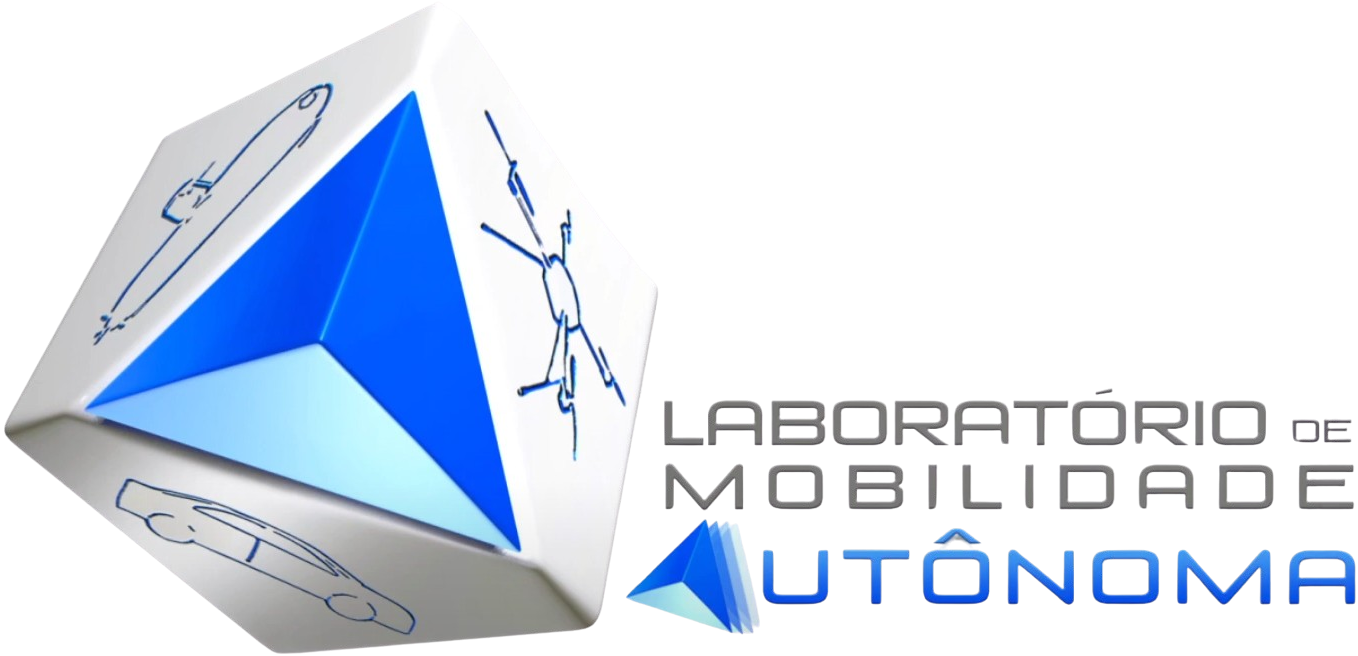
\includegraphics[width=0.5\linewidth]{img/core/Logo_LMA.png}
	\end{figure}
	
\end{frame}

\end{document}
